\caulc
\begin{ex}%[1D6H3-3]%[Dự án đề tinh hoa THPT 2026 - Thầy Ái TDM]%[Lê Phúc]
	Tập giá trị của hàm số $y=\log_{2}(1-x)$ là
	\choice
	{$(-\infty;1)$}
	{$\mathbb{R}\setminus\{1\}$}
	{\True $(-\infty;+\infty)$}
	{$(1;+\infty)$}
	\loigiai{
		Tập giá trị của hàm số $y=\log_{2}(1-x)$ là $\mathbb{R}=(-\infty;+\infty)$.
	}
\end{ex}

\begin{ex}%[1D6H4-3]%[Dự án đề tinh hoa THPT 2026 - Thầy Ái TDM]%[Lê Phúc]
	Nghiệm của bất phương trình $2^{x^2-x+1}\le8$ là
	\choice
	{$0<x\le2$}
	{$x\le-1$}
	{$x\ge3$}
	{\True $-1\le x\le2$}
	\loigiai{
		Ta có bất phương trình đã cho tương đương với
		\allowdisplaybreaks
		\begin{eqnarray*}
			&&2^{x^{2}-x+1}\le2^3\\
			&\Leftrightarrow&x^2-x+1\le3\\
			&\Leftrightarrow&x^2-x-2\le0\\
			&\Leftrightarrow&-1\le x\le2.
		\end{eqnarray*}
		Vậy nghiệm của bất phương trình là $-1\le x\le2$.
	}
\end{ex}

\begin{ex}%[1H8H7-2]%[Dự án đề tinh hoa THPT 2026 - Thầy Ái TDM]%[Lê Phúc]
	\immini[thm]{Cho hình chóp $S. ABC$ có đáy $ABC$ là tam giác đều cạnh $a$ và khoảng cách từ đỉnh $S$ xuống đáy $(ABC)$ bằng $3a$. Thể tích khối chóp $S. ABC$ bằng
		\choice
		{$\dfrac{a^{3}\sqrt{3}}{6}$}
		{$\dfrac{a^{3}\sqrt{2}}{12}$}
		{\True $\dfrac{a^{3}\sqrt{3}}{4}$}
		{$\dfrac{a^{3}\sqrt{6}}{9}$}}
	{\begin{tikzpicture}[scale=0.8, font=\footnotesize, line join=round, line cap=round, >=stealth]
			\coordinate (A) at (-2,0);
			\coordinate (B) at (-1,-3);
			\coordinate (C) at (3,0);
			\coordinate (M) at ($(A)!0.5!(B)$);
			\coordinate (H) at ($(C)!2/3!(M)$);
			\coordinate (S) at ($(H)+(0,5)$);
			\draw(S)--(A) (S)--(B) (S)--(C) (B)--(C);
			\draw[dashed](A)--(C);
			\foreach \i/\g in {S/90,A/180,B/-90,C/0,H/-70}{\draw[fill=black](\i) circle (1pt) ($(\i)+(\g:3mm)$) node[scale=1]{$\i$};}
			\draw[dashed](S)--(H)node[right,pos=0.5]{$3a$};
			\draw(A)--(B)node[left,pos=0.5]{$a$};
	\end{tikzpicture}}
	\loigiai{
		Diện tích đáy $ABC$ là $S_{\triangle ABC}=\dfrac{a^2\sqrt{3}}{4}$.\\
		Khoảng cách từ đỉnh $S$ xuống đáy $(ABC)$ chính là chiều cao $h=3a$.\\
		Thể tích khối chóp $S. ABC$ là
		\[V=\dfrac{1}{3} \cdot S_{\triangle ABC} \cdot h = \dfrac{1}{3} \cdot \dfrac{a^2\sqrt{3}}{4} \cdot 3a = \dfrac{a^3\sqrt{3}}{4}.\]
	}
\end{ex}

\begin{ex}%[1D3H2-3]%[Dự án đề tinh hoa THPT 2026 - Thầy Ái TDM]%[Lê Phúc]
	Giá trị $\lim\limits_{x\to-\infty}\dfrac{\sqrt{x^{2}-3^{2\,026}}-x}{x+1}$ bằng
	\choice
	{$0$}
	{$+\infty$}
	{$1$}
	{\True $-2$}
	\loigiai{
		Ta có
		\allowdisplaybreaks
		\begin{eqnarray*}
			\lim\limits_{x\to-\infty}\dfrac{\sqrt{x^2-3^{2\,026}}-x}{x+1}
			&=&\lim\limits_{x\to-\infty}\dfrac{-x\sqrt{1-\dfrac{3^{2\,026}}{x^2}}-x}{x+1}\\
			&=&\lim\limits_{x\to-\infty}\dfrac{-\sqrt{1-\dfrac{3^{2\,026}}{x^2}}-1}{1+\dfrac{1}{x}}\\
			&=&-2.
		\end{eqnarray*}
	}
\end{ex}

\begin{ex}%[2D1N1-2]%[Dự án đề tinh hoa THPT 2026 - Thầy Ái TDM]%[Lê Phúc]
	\immini[thm]{Cho đồ thị của hàm số $y=f(x)$ như hình vẽ bên. Hỏi hàm số $f(x)$ nghịch biến trên khoảng nào dưới đây?
		\choice
		{$(-5;+\infty)$}
		{\True $(-1;4)$}
		{$(4;+\infty)$}
		{$(-\infty;4)$}}
	{\begin{tikzpicture}[>=stealth,yscale=.5,xscale=0.7,font=\footnotesize,line join=round,line cap=round]
			\tikzset{every node/.style={scale=1.3}}
			\def\xmin{-6} \def\xmax{6.78}
			\def\ymin{-2} \def\ymax{8.7}
			
			% --- Hệ trục tọa độ ---
			\draw[->] (\xmin,0)--(0,0)node[below right]{$O$}--(\xmax,0)node[below]{$x$};
			\draw[->] (0,\ymin)--(0,\ymax)node[right]{$y$};
			
			% --- Đồ thị f(x)=0.1*(x+4)*(x-4)^2 ---
			% Cực đại thật tại x=-4/3, f(-4/3)≈7.59
			% Cắt Ox thật tại -4 (nhãn giả -5); cực tiểu chạm Ox tại 4
			\begin{scope}
				\clip (\xmin,\ymin) rectangle (\xmax,\ymax);
				\draw[samples=200,domain=-6:6.78,smooth,variable=\x,blue]
				plot (\x,{0.1*((\x)^3)+-0.4*((\x)^2)+-1.6*(\x)+6.4});
			\end{scope}
			
			% --- Các điểm đặc biệt ---
			\fill (-4,0) circle (2.5pt) node[above left] {$-5$};
			\fill (4,0) circle (2.5pt) node[below] {$4$};
			\fill (-1.333,7.585) circle (2.5pt);
			\fill (-1.333,0) circle (2.5pt) node[below] {$-1$};
			\draw[dashed] (-1.333,0)--(-1.333,7.585);
			
			\path (5.3,4.2) node[left] {$f(x)$};
	\end{tikzpicture}}
	\loigiai{
		Dựa vào đồ thị hàm số, ta thấy trên khoảng $(-1;4)$, đồ thị đi xuống từ trái sang phải.\\
		Do đó, hàm số $y=f(x)$ nghịch biến trên khoảng $(-1;4)$.
	}
\end{ex}

\begin{ex}%[2H2N2-3]%[Dự án đề tinh hoa THPT 2026 - Thầy Ái TDM]%[Lê Phúc]
	Trong không gian $Oxyz$, cho hai vectơ $\overrightarrow{u}=(1;2;0)$, $\overrightarrow{v}=(-2;1;-1)$. Tổng của hai vectơ này có tọa độ là
	\choice
	{$(3;1;1)$}
	{\True $(-1;3;-1)$}
	{$(-3;-1;-1)$}
	{$(1;-2;1)$}
	\loigiai{
		Ta có $\overrightarrow{u}+\overrightarrow{v} = \left(1+(-2); 2+1; 0+(-1)\right) = (-1;3;-1)$.
	}
\end{ex}

\begin{ex}%[2D4N1-4]%[Dự án đề tinh hoa THPT 2026 - Thầy Ái TDM]%[Lê Phúc]
	Họ nguyên hàm của hàm số $f(x)=\mathrm{e}^{x}+1$ là
	\choice
	{$F(x)=\mathrm{e}^{x}+1$}
	{$F(x)=-\mathrm{e}^{x}+x+C$}
	{$F(x)=\mathrm{e}^{x}+C$}
	{\True $F(x)=\mathrm{e}^{x}+x+C$}
	\loigiai{
		Ta có
		$F(x)=\displaystyle\int\limits f(x)\mathrm{\,d}x =\displaystyle\int\limits \left(\mathrm{e}^x+1\right)\mathrm{d}x = \mathrm{e}^x+x+C$.
	}
\end{ex}

\begin{ex}%[2H5N2-2]%[Dự án đề tinh hoa THPT 2026 - Thầy Ái TDM]%[Lê Phúc]
	Trong không gian $Oxyz$, đường thẳng $d\colon \dfrac{x-1}{3}=\dfrac{y}{4}=\dfrac{z-1}{2}$ có vectơ chỉ phương là
	\choice
	{$\overrightarrow{u}_1=(1;0;1)$}
	{$\overrightarrow{u}_2=(1;-3;2)$}
	{$\overrightarrow{u}_3=(3;2;4)$}
	{\True $\overrightarrow{u}_4=(3;4;2)$}
	\loigiai{
		Một vectơ chỉ phương của $d$ là $\overrightarrow{u}_4=(3;4;2)$.
	}
\end{ex}

\begin{ex}%[2D4H3-1]%[Dự án đề tinh hoa THPT 2026 - Thầy Ái TDM]%[Lê Phúc]
	Cho hình phẳng $(H)$ giới hạn bởi các đường $f(x)=x^{2}+1$; $g(x)=3x-1$. Diện tích hình phẳng $(H)$ bằng
	\choice
	{\True $\dfrac{1}{6}$}
	{$\dfrac{2}{3}$}
	{$\dfrac{1}{3}$}
	{$\dfrac{\pi}{2}$}
	\loigiai{
		Phương trình hoành độ giao điểm của hai đồ thị hàm số là
		\[x^2+1=3x-1 \Leftrightarrow x^2-3x+2=0 \Leftrightarrow \hoac{&x=1\\&x=2.}\]
		Diện tích hình phẳng $(H)$ là
		\[S =\displaystyle\int\limits_{1}^{2} \left|\left(x^2+1\right)-(3x-1)\right|\mathrm{\,d}x=\displaystyle\int\limits_{1}^{2} \left|x^2-3x+2\right|\mathrm{\,d}x=\dfrac{1}{6}.\]
	}
\end{ex}

\begin{ex}%[2H2H1-2]%[Dự án đề tinh hoa THPT 2026 - Thầy Ái TDM]%[Lê Phúc]
	\immini[thm]{Cho hình hộp $ABCD. A'B'C'D'$. Tổng $\overrightarrow{AB}+\overrightarrow{A'D'}+\overrightarrow{DD'}$ bằng vectơ nào dưới đây
		\choice
		{$\overrightarrow{AB'}$}
		{\True $\overrightarrow{AC'}$}
		{$\overrightarrow{0}$}
		{$\overrightarrow{BD}$}}
	{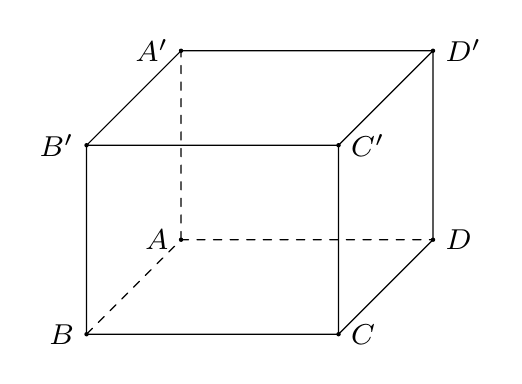
\begin{tikzpicture}[scale=0.8, font=\footnotesize, line join=round, line cap=round, >=stealth]
			\coordinate (A) at (0,0);
			\coordinate (B) at (-1.5,-1.5);
			\coordinate (C) at (2.5,-1.5);
			\coordinate (D) at (4,0);
			\coordinate (A') at (0,3);
			\coordinate (B') at (-1.5,1.5);
			\coordinate (C') at (2.5,1.5);
			\coordinate (D') at (4,3);
			\draw[dashed] (B)--(A)--(D) (A)--(A');
			\draw (A')--(B')--(C')--(D')--cycle;
			\draw (B')--(B)--(C)--(D)--(D') (C)--(C');
			\fill (A) circle (1pt) node[left] {$A$};
			\fill (B) circle (1pt) node[left] {$B$};
			\fill (C) circle (1pt) node[right] {$C$};
			\fill (D) circle (1pt) node[right] {$D$};
			\fill (A') circle (1pt) node[left] {$A'$};
			\fill (B') circle (1pt) node[left] {$B'$};
			\fill (C') circle (1pt) node[right] {$C'$};
			\fill (D') circle (1pt) node[right] {$D'$};
	\end{tikzpicture}}
	\loigiai{
		Vì $ABCD. A'B'C'D'$ là hình hộp nên ta có $\overrightarrow{A'D'} = \overrightarrow{AD}$ và $\overrightarrow{DD'} = \overrightarrow{AA'}$.\\
		Ta có
		$\overrightarrow{AB}+\overrightarrow{A'D'}+\overrightarrow{DD'} = \overrightarrow{AB}+\overrightarrow{AD}+\overrightarrow{AA'}=\overrightarrow{AC'}$.
	}
\end{ex}

\begin{ex}%[2D1H4-1]%[Dự án đề tinh hoa THPT 2026 - Thầy Ái TDM]%[Lê Phúc]
	Cho hàm số $y=\dfrac{x^{2}+2x-3}{x^{2}-5x+4}$ có đồ thị $(C)$. Số đường tiệm cận của đồ thị $(C)$ là
	\choice
	{\True $2$}
	{$3$}
	{$1$}
	{$0$}
	\loigiai{
		Tập xác định $\mathcal{D} = \mathbb{R}\setminus\{1;4\}$.\\
		Ta có $y=\dfrac{x^2+2x-3}{x^2-5x+4}= \dfrac{(x-1)(x+3)}{(x-1)(x-4)}=\dfrac{x+3}{x-4}$.\\
		Ta có $\lim\limits_{x\to\pm\infty} y = \lim\limits_{x\to\pm\infty} \dfrac{x+3}{x-4} = 1$.\\
		Suy ra $y=1$ là một tiệm cận ngang của đồ thị hàm số.\\
		Ta lại có
		\begin{itemize}
			\item $\lim\limits_{x\to 4^+} y=\lim\limits_{x\to 4^+}\dfrac{x+3}{x-4}=+\infty$.\item $\lim\limits_{x\to 4^-} y=\lim\limits_{x\to 4^-}\dfrac{x+3}{x-4}=-\infty$.
		\end{itemize}
		Suy ra $x=4$ là một tiệm cận đứng của đồ thị $(C)$.\\
		Ta có $\lim\limits_{x\to1} y = \dfrac{1+3}{1-4} = -\dfrac{4}{3}$.\\
		Suy ra $x=1$ không phải là tiệm cận đứng của đồ thị hàm số.\\
		Vậy đồ thị $(C)$ có tổng cộng $2$ đường tiệm cận.
	}
\end{ex}

\begin{ex}%[2D3H1-2]%[Dự án đề tinh hoa THPT 2026 - Thầy Ái TDM]%[Lê Phúc]
	Cho mẫu số liệu ghép nhóm $M_{1}$ cùng có $7$ nhóm (các nhóm trong mỗi mẫu số liệu bằng nhau), có phần tử đại diện của nhóm thứ $6$ hơn nhóm thứ $4$ một lượng là $4$. Khoảng biến thiên của $M_1$ bằng
	\choice
	{$7$}
	{\True $14$}
	{$13$}
	{$16$}
	\loigiai{
		Gọi độ dài của mỗi nhóm là $h$. \\
		Phần tử đại diện của nhóm thứ $i$ được tính bằng trung điểm của nhóm đó. \\
		Khoảng cách giữa hai phần tử đại diện liên tiếp chính bằng độ dài $h$ của một nhóm.\\
		Ta có phần tử đại diện của nhóm thứ $6$ hơn nhóm thứ $4$ một lượng là $4$, tức là
		\[x_6 - x_4 = 2h = 4 \Rightarrow h = 2.\]
		Mẫu số liệu có tất cả $7$ nhóm bằng nhau, khoảng biến thiên của mẫu số liệu ghép nhóm là
		\[R = x_{\max} - x_{\min} = 7 \cdot h = 7 \cdot 2 = 14.\]
	}
\end{ex}
\cauds
\begin{ex}%[2D1H3-2]%[Dương Công Tạo]
	Trong mặt phẳng toạ độ $Oxy$, cho hàm số $y=x-2\,027\ln(x-1)$ có đồ thị $(C)$.
	\choiceTF
	{\True Tập xác định của hàm số là $\mathscr{D} = (1;+\infty)$}
	{\True $f'(x)=1-\dfrac{2\,027}{x-1}$}
	{\True $(C)$ có đúng một điểm cực tiểu}
	{\True Giá trị nhỏ nhất của $f(x)$ làm tròn kết quả đến hàng đơn vị là $-13\,406$}
	\loigiai{
		\begin{itemchoice}
			\itemch Hàm số $y=x-2\,027\ln(x-1)$ xác định khi và chỉ khi $x-1>0\Leftrightarrow x>1$.\\
			Vậy tập xác định của hàm số là $\mathscr{D} = (1;+\infty)$.
			\itemch Với $x>1$, ta có $y'=1-\dfrac{2\,027}{x-1}=\dfrac{x-2\,028}{x-1}$.
			\itemch Ta có $y'=0\Leftrightarrow x=2\,028$.\\
			Bảng biến thiên
			\begin{center}
				
\begin{tikzpicture}[>=stealth]
					\tkzTabInit[nocadre=false,lgt=1.5,espcl=2,deltacl=0.6]{$x$/.7 ,$y'$/.7,$y$/2}
					{$1$ , $2\,028$ , $+\infty$}
					\tkzTabLine{ , - , $0$ , + , }
					\tkzTabVar{+/$+\infty$ , -/$y_{\text{CT}}$ , +/$+\infty$}
				\end{tikzpicture}
			\end{center}
			Dựa vào bảng biến thiên, ta thấy đồ thị $(C)$ có đúng một điểm cực tiểu.
			\itemch Dựa vào bảng biến thiên, ta có $\min\limits_{(1;+\infty)}y=2\,028-2\,027\ln 2\,027\approx-13\,406$ (\textit{làm tròn kết quả đến hàng đơn vị}).
		\end{itemchoice}
	}
\end{ex}

\begin{ex}%[TDMZZ29]%[Hà Văn Hảo]%[2D6V2-4]
	Người ta thiết kế một con súc sắc cân đối đồng chất có dạng đa diện 12 mặt đều, trên đó có ba mặt $3$ chấm, bốn mặt $4$ chấm và năm mặt $5$ chấm. Tiến hành gieo ngẫu nhiên con súc sắc này hai lần liên tiếp. Gọi $A$ là biến cố lần thứ nhất xuất hiện mặt $5$ chấm, $B$ là biến cố tổng số chấm ở hai lần gieo bằng $9$.
	\choiceTF
	{\True $\mathrm{P}(A) = \dfrac{5}{12}$}
	{\True $\mathrm{P}(B \mid A) = \dfrac{1}{3}$}
	{ $\mathrm{P}(B) = \dfrac{5}{24}$}
	{ $\mathrm{P}(A \mid B) = \dfrac{7}{24}$}
	\loigiai{
		Xác suất xuất hiện các mặt trong mỗi lần gieo là
		\begin{itemize}
			\item Xác suất xuất hiện mặt $3$ chấm là $\mathrm{P}(3c) = \dfrac{3}{12} = \dfrac{1}{4}$.
			\item Xác suất xuất hiện mặt $4$ chấm là $\mathrm{P}(4c) = \dfrac{4}{12} = \dfrac{1}{3}$.
			\item Xác suất xuất hiện mặt $5$ chấm là $\mathrm{P}(5c) = \dfrac{5}{12}$.
		\end{itemize}
		\begin{itemchoice}
			\itemch Biến cố $A$: \lq\lq Lần thứ nhất xuất hiện mặt $5$ chấm\rq\rq.\\
			Xác suất của biến cố $A$ là $\mathrm{P}(A) = \dfrac{5}{12}$.
			\itemch Biến cố $B\mid A$ là biến cố \lq\lq Tổng số chấm ở hai lần gieo bằng $9$ với điều kiện lần thứ nhất đã xuất hiện mặt $5$ chấm\rq\rq.\\
			Khi lần thứ nhất đã ra mặt $5$ chấm, để tổng số chấm bằng $9$ thì lần thứ hai bắt buộc phải xuất hiện mặt $4$ chấm.\\
			Vì hai lần gieo độc lập nên $\mathrm{P}(B\mid A) = \dfrac{4}{12} = \dfrac{1}{3}$.
			\itemch Biến cố $B$ \lq\lq Tổng số chấm ở hai lần gieo bằng $9$\rq\rq.\\
			Các cặp số chấm ở lần một và lần hai thỏa mãn là $(4;5)$ và $(5;4)$.\\
			Xác suất của biến cố $B$ là
			\[\mathrm{P}(B) = \dfrac{4}{12} \cdot \dfrac{5}{12} + \dfrac{5}{12} \cdot \dfrac{4}{12} = \dfrac{5}{36} + \dfrac{5}{36} = \dfrac{5}{18}.\]
			\itemch Theo công thức xác suất điều kiện, ta có
			\[\mathrm{P}(A\mid B) = \dfrac{\mathrm{P}(A)\mathrm{P}(B\mid A)}{\mathrm{P}(B)}= \dfrac{\dfrac{5}{12} \cdot \dfrac{4}{12}}{\dfrac{5}{18}}=\dfrac{1}{2}.\]
		\end{itemchoice}
	}
\end{ex}

\begin{ex}%[2H2V2-6]%[TDMZZ29]%[Vũ Hồng Toàn]
	Trong không gian $Oxyz$, đơn vị dài trên mỗi trục là kilomet và đơn vị vận tốc là km/h. Ở thời điểm ban đầu, một vật chuyển động thẳng đều từ điểm $A(2;3;0)$ chuyển động theo vectơ vận tốc $\vec{u} = (3;-4;1)$ trong khoảng thời gian $3$ giờ thì gặp một cơn gió nhẹ đổi hướng chuyển động theo vectơ vận tốc $\vec{v} = (5;-3;1)$.
	\begin{center}
		\begin{tikzpicture}[scale=1, font=\footnotesize, line join=round, line cap=round, >=stealth]
			\tikzset{declare function={a=1.5;goc=30;}}
			\path (0.6,0.2)coordinate (A) ++(goc:a)coordinate (B)++(goc:0.8*a)coordinate (C)++(goc+20:0.7*a)coordinate (D)++(goc+20:0.9*a)coordinate (E);
			% Các trục tọa độ
			\draw[->] (0,0) -- (-1.5,-1.5) node[left] {$x$};
			\draw[->] (0,0) -- (4.5,0) node[below] {$y$};
			\draw[->] (0,0) -- (0,3.5) node[right] {$z$};
			\node[left] at (0,0) {$O$};
			\fill (0,0) circle (1.5pt);
			\fill (A) circle (1.5pt) node[above left] {$A$};
			\draw[dashed] (B)--(C) (D)--(E);
			\draw[thick,->] (A) -- (B) node[below right,pos=0.5] {$\vec{u}$};
			\draw[thick,blue,->] (C) -- (D) node[below right,pos=0.5] {$\vec{v}$};
		\end{tikzpicture}
	\end{center}
	\choiceTF
	{\True Tốc độ chuyển động của vật trong $3$ giờ đầu bằng $\sqrt{26}$ km/h}
	{Toạ độ của vật ở thời điểm $t_1 = 3$\,h là $(9;-12;3)$}
	{\True Toạ độ của vật sau $8$ giờ là $(36;-24;8)$}
	{Khi vừa đạt độ cao $10$\,km thì vật đã lệch so với vị trí dự định ban đầu sẽ đến (với cùng khoảng thời gian như nhau) là $\sqrt{322}$\,km}
	\loigiai{
		\begin{itemchoice}
			\itemch Trong $3$ giờ đầu, vật chuyển động với vectơ vận tốc $\vec{u} = (3;-4;1)$.\\
			Tốc độ chuyển động của vật trong giai đoạn này là độ dài của vectơ vận tốc
			\[v_1 = \left|\vec{u}\right| = \sqrt{3^2 + (-4)^2 + 1^2} = \sqrt{26} \text{ (km/h)}.\]
			\itemch Vật xuất phát từ điểm $A(2;3;0)$.\\ Sau $3$ giờ chuyển động với vận tốc $\vec{u} = (3;-4;1)$, toạ độ của vật tại thời điểm $t_1 = 3\text{h}$ là
			\[\vec{OM} = \vec{OA} + 3\vec{u} = \left(2;3;0\right) + 3\cdot\left(3;-4;1\right) = \left(11;-9;3\right).\]
			Do đó, toạ độ của vật lúc này là $M(11;-9;3)$.
			\itemch Tại thời điểm $t_1 = 3$\,h, vật ở vị trí $M(11;-9;3)$.\\
			Trong $5$ giờ tiếp theo (để đủ $8$ giờ), vật chuyển động với vận tốc $\vec{v} = (5;-3;1)$.\\
			Toạ độ của vật sau $8$ giờ là
			\[\vec{ON} = \vec{OM} + 5\vec{v} = \left(11;-9;3\right) + 5\cdot\left(5;-3;1\right) = \left(36;-24;8\right).\]
			Do đó, toạ độ của vật sau $8$ giờ là $N(36;-24;8)$.
			\itemch Gọi $z(t)$ là độ cao (cao độ) của vật tại thời điểm $t$ (giờ).
			\begin{itemize}
				\item Với $0 \le t \le 3$: cao độ của vật là $z(t) = 0 + 1 \cdot t = t$. Tại $t=3$, cao độ là $3$ km.
				\item Với $t > 3$: cao độ của vật là $z(t) = 3 + 1 \cdot (t-3) = t$.
			\end{itemize}
			Như vậy, cao độ của vật tại thời điểm $t$ luôn là $z(t) = t$\,(km).\\
			Vật đạt độ cao $10$ km tại thời điểm $t = 10$ giờ.\\
			Tại thời điểm $t = 10$ giờ
			\begin{itemize}
				\item Vị trí thực tế của vật là
				\[\vec{OP} = \vec{OA} + 3\vec{u} + 7\vec{v} = (2;3;0) + (9;-12;3) + (35;-21;7) = (46;-30;10).\]
				Suy ra $P(46;-30;10)$.
				\item Vị trí dự định của vật nếu không đổi hướng (vẫn chuyển động với vận tốc $\vec{u}$) là
				\[\vec{OQ} = \vec{OA} + 10\vec{u} = (2;3;0) + 10\cdot (3;-4;1) = (32;-37;10).\]
				Suy ra $Q(32;-37;10)$.
			\end{itemize}
			Khoảng cách lệch giữa vị trí thực tế và vị trí dự định là
			\[PQ = \sqrt{(-14)^2 + (-7)^2+0^2} = \sqrt{245} \text{ (km)}.\]
		\end{itemchoice}
	}
\end{ex}

\begin{ex}%[2D4V2-6]%[TDMZZ29]%[Văn Minh Thoại]
	Một vật bắt đầu chuyển động thẳng từ địa điểm $A$ đến dừng lại tại địa điểm $B$ theo hàm vận tốc
	\[v(t) =\heva{&at^2 + b && 0 \le t < 20 \\& 20 & &20 \le t \le 60 \\ &mt + n && 60 \le t \le 100} \mathrm{\,(m/s)}.\]
	Trong đó thời gian $t$ tính theo giây, gốc thời gian tính từ $A$.
	\choiceTF
	{\True $a=0{,}05$; $b=0$}
	{\True Quãng đường vật đi được trong $20$ giây đầu là $133$ m \textit{(làm tròn kết quả đến hàng đơn vị)}}
	{Tổng quãng đường vật đi được tính từ $A$ đến ngay trước khi vật giảm tốc độ dài hơn $1\,000$ m}
	{\True Độ dài quãng đường $AB$ bằng $1\,333$ m \textit{(làm tròn kết quả đến hàng đơn vị)}}
	\loigiai{
		Vì vật bắt đầu chuyển động từ $A$ tại $t=0$ nên $v(0)=0\Rightarrow a\cdot 0^2+b=0\Rightarrow b=0$.\\
		Vì vận tốc của vật là một đại lượng vật lý thay đổi liên tục theo thời gian nên hàm số $v(t)$ liên tục trên đoạn $[0;100]$. Ta có
		\begin{itemize}
			\item $\lim\limits_{t \to 20^-} v(t) = v(20) \Leftrightarrow a \cdot 20^2 + b = 20 \Rightarrow 400a = 20 \Rightarrow a = 0{,}05$.
			\item $\lim\limits_{t \to 60^+} v(t) = v(60) \Leftrightarrow m \cdot 60 + n = 20$. \quad ($1$)
		\end{itemize}
		Khi vật dừng lại tại $B$ tương ứng với $t=100$, ta có
		\[v(100)=0\Rightarrow 100m+n=0\quad(2).\]
		Từ $(1)$ và $(2)$ ta có hệ phương trình
		\[ \heva{& 60m+n=20 \\ & 100m+n=0} \Leftrightarrow \heva{& m=-0{,}5 \\ & n=50.} \]
		Vậy hàm vận tốc của vật là $v(t)=\heva{& 0{,}05t^2&& 0\le t<20 \\ & 20&& 20\le t\le 60 \\ & -0{,}5t+50&& 60\le t\le 100.}$
		\begin{center}
			\begin{tikzpicture}[line join=round,line cap=round,>=stealth,scale=0.1]
				\draw[->] (-10,0) -- (115,0) node[below] {$t\mathrm{\,(s)}$};
				\draw[->] (0,-5) -- (0,30) node[left] {$v\mathrm{\,(m/s)}$};
				\fill (0,0) circle (15pt) node[below left] {$O$};
				\draw[thick,blue,domain=0:20,samples=100] plot (\x,{0.05*(\x)^2});
				\draw[thick,blue] (20,20) -- (60,20);
				\draw[thick,blue] (60,20) -- (100,0);
				\draw[dashed] (20,0) node[below] {$20$} -- (20,20);
				\draw[dashed] (60,0) node[below] {$60$} -- (60,20);
				\draw[dashed] (0,20) node[left] {$20$} -- (20,20);
				\fill (100,0) circle (15pt) node[below] {$100$};
				\node at (50,25) [blue] {Đồ thị biểu diễn vận tốc $v (t)$};
			\end{tikzpicture}
		\end{center}
		\begin{itemchoice}
			\itemch Ta tìm được $a=0{,}05$ và $b=0$.
			\itemch Quãng đường vật đi được trong $20$ giây đầu là
			\[ s_1 = \displaystyle\int\limits_{0}^{20} 0{,}05t^2 \mathrm{\,d}t = \left. \left( \dfrac{0{,}05t^3}{3} \right) \right|_0^{20} = \dfrac{400}{3} \approx 133\mathrm{\,m}. \]
			\itemch Thời điểm vật bắt đầu giảm tốc độ là $t=60$. Tổng quãng đường vật đi được tính từ $A$ đến ngay trước khi vật giảm tốc độ là
			\[ S_{60} = s_1 + \displaystyle\int\limits_{20}^{60} 20 \mathrm{\,d}t = \dfrac{400}{3}+800=\dfrac{2\,800}{3} \approx 933{,}33<1\,000\mathrm{\,m}. \]
			\itemch Quãng đường vật đi được trong giai đoạn giảm tốc độ (từ $t=60$ đến $t=100$) là
			\[ s_3 = \displaystyle\int\limits_{60}^{100} (-0{,}5t + 50) \mathrm{\,d}t = 400\mathrm{\,m}. \]
			Độ dài quãng đường $AB$ là tổng quãng đường vật đi được trong $100$ giây là
			\[ S_{AB} = S_{60} + s_3 = \dfrac{2\,800}{3} + 400 = \dfrac{4\,000}{3} \approx 1\,333\mathrm{\,m}. \]
		\end{itemchoice}
	}
\end{ex}
\caukq 
\begin{ex}%[1H3V4-3]%[TDMZZ29]%[Lê Hồ Quang Minh]
	Cho hình lăng trụ $ABC. A'B'C'$ có $AA'=8$, $AB=6$, $AC=8$, $\widehat{BAC}=45^\circ$. Biết hình chiếu vuông góc của đỉnh $A$ lên mặt phẳng $(A'B'C')$ là trung điểm của cạnh $B'C'$. Hãy tính thể tích khối lăng trụ $ABC. A'B'C'$ \textit{(không làm tròn ở các phép tính trung gian và làm tròn kết quả cuối cùng đến hàng phần mười)}?
	\par\shortans[0]{114,3}
	\loigiai{
		\immini{
			Diện tích tam giác đáy $ABC$ được tính bởi công thức
			\[S_{ABC} = \dfrac{1}{2} \cdot AB \cdot AC \cdot \sin\widehat{BAC} = \dfrac{1}{2} \cdot 6 \cdot 8 \cdot \sin 45^\circ = 12\sqrt{2}.\]
			Áp dụng định lý côsin trong tam giác $ABC$, ta có
			\allowdisplaybreaks
			\begin{eqnarray*}
				B'C'^2 = BC^2 &=& AB^2 + AC^2 - 2\cdot AB \cdot AC \cdot \cos\widehat{BAC} \\
				&=& 6^2 + 8^2 - 2 \cdot 6 \cdot 8 \cdot \cos 45^\circ \\
				&=& 100 - 48\sqrt{2}.
			\end{eqnarray*}
		}{
			\begin{tikzpicture}[scale=0.8, font=\footnotesize, line join=round, line cap=round, >=stealth]
				\path 
				(0,0) coordinate (A')
				++(-50:2.5) coordinate (B')
				(5,0) coordinate (C')
				($(B')!0.5!(C')$) coordinate (H)
				($(H)+(0,4.8)$) coordinate (A)
				($(B')+(A)-(A')$) coordinate (B)
				($(C')+(A)-(A')$) coordinate (C)
				;
				\draw (B')--(C') (A)--(B)--(C)--cycle (B)--(B') (C)--(C') (A)--(A')--(B');
				\draw[dashed] (A)--(H)--(A')--(C');
				\pic[draw,thin,angle radius=2mm] {right angle = A--H--A'};
				\foreach \i/\g in {A'/135,B'/-90,C'/-45,A/135,B/-135,C/-45,H/-90}
				\fill[black] (\i) circle(1pt)+(\g:3mm)node[scale=0.95]{$\i$};
			\end{tikzpicture}
		}
		\noindent
		Gọi $H$ là trung điểm của $B'C'$. Theo giả thiết, $AH \perp (A'B'C')$.\\
		Trong tam giác $A'B'C'$, $A'H$ là đường trung tuyến nên
		\allowdisplaybreaks
		\begin{eqnarray*}
			A'H^2 &=& \dfrac{2\cdot\left(A'B'^2 + A'C'^2\right) - B'C'^2}{4}\\
			&=& \dfrac{2\cdot\left(6^2 + 8^2\right) - \left(100 - 48\sqrt{2}\right)}{4} \\
			&=& \dfrac{200 - 100 + 48\sqrt{2}}{4} = 25 + 12\sqrt{2}.
		\end{eqnarray*}
		Xét tam giác $AA'H$ vuông tại $H$ có $AH = \sqrt{AA'^2 - A'H^2} = \sqrt{8^2 - \left(25 + 12\sqrt{2}\right)} = \sqrt{39 - 12\sqrt{2}}$.\\
		Vậy thể tích khối lăng trụ $ABC. A'B'C'$ là
		\[V = AH \cdot S_{ABC} = 12\sqrt{2}\cdot \sqrt{39 - 12\sqrt{2}} \approx 79,7.\]
	}
\end{ex}
\begin{ex}
	content
\end{ex}
\begin{ex}%[2D1V3-6]%[TDMZZ29-19-TLN]%[Đỗ Đường Hiếu]
	\immini[thm]{
		Một chiếc đèn pin tại vị trí $S$ chiếu chùm sáng phân kì với góc chiếu sáng $\widehat{ASC} = 60^\circ$ không đổi, sang phía góc $xBy$ như hình vẽ bên dưới. Biết $\widehat{SBA} = 60^\circ$, $\widehat{SBC} = 45^\circ$, $SB = 6$ m. Với điều kiện $A$ luôn thuộc tia $Bx$ và $C$ luôn thuộc tia $By$ thì tổng độ dài hai đoạn $BA$ và $BC$ tính theo đơn vị mét lớn nhất bằng bao nhiêu (\textit{làm tròn kết quả đến hàng phần trăm})?}
	{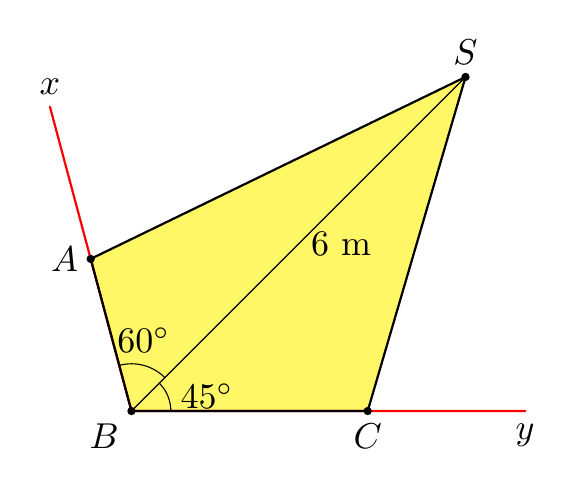
\begin{tikzpicture}[scale=1, font=, line join=round, line cap=round, >=stealth]
			\path 
			(0:0) coordinate (B)
			(105:4) coordinate (x)
			(0:5) coordinate (y)
			(45:6) coordinate (S)
			(105:2) coordinate (A)
			(0:3) coordinate (C)
			;
			\fill[yellow!60] (S) -- (A) -- (B) -- (C) -- cycle;
			\draw[thick, red] (x) -- (B) -- (y);
			\draw[thick] (S) -- (A) -- (B) -- (C) -- (S);
			\draw (S) -- (B) node[midway, right] {$6$ m};
			\draw (0.5,0) arc (0:45:0.5) node[midway, right] {$45^\circ$};
			\draw (105:0.6) arc (105:45:0.6) node[midway, above] {$60^\circ$};
			\fill (S) circle (1.5pt) node[above] {$S$};
			\fill (A) circle (1.5pt) node[left] {$A$};
			\fill (B) circle (1.5pt) node[below left] {$B$};
			\fill (C) circle (1.5pt) node[below] {$C$};
			\draw (x) node[above] {$x$};
			\draw (y) node[below] {$y$};
		\end{tikzpicture}
	}
	\par\shortans{6,19}
	\loigiai{
		Đặt $BA = a$ và $BC = c$. \\
		Ta có $\widehat{ASC} = \dfrac{\pi}{3}$, $\widehat{SBA} = \dfrac{\pi}{3}$, $\widehat{SBC} = \dfrac{\pi}{4}$.\\
		Đặt $\widehat{ASB}=\alpha$, suy ra $\widehat{BSC}=\dfrac{\pi}{3}-\alpha$, $\widehat{SAB}=\dfrac{2\pi}{3}-\alpha$ và $\widehat{SCB}=\dfrac{5\pi}{12}+\alpha$.\\
		Trong tam giác $SBA$, theo định lý hàm số sin, ta có
		$$\dfrac{BA}{\sin\widehat{BSA}} = \dfrac{SB}{\sin\widehat{SAB}}=\dfrac{6}{\sin \left(\dfrac{2\pi}{3}-\alpha\right)}\Rightarrow BA=6\cdot\dfrac{\sin\alpha}{\sin \left(\dfrac{2\pi}{3}-\alpha\right)}.$$
		Trong tam giác $SBC$, theo định lý hàm số sin, ta có
		$$\dfrac{BC}{\sin\widehat{BSC}} = \dfrac{SB}{\sin \widehat{SCB}}=\dfrac{6}{\sin\left(\dfrac{5\pi}{12}+\alpha\right)}\Rightarrow BC=6\cdot \dfrac{\sin \left(\dfrac{\pi}{3}-\alpha\right)}{\sin\left(\dfrac{5\pi}{12}+\alpha\right)}.$$
		Do đó
		$$BA+BC=6\cdot \left[\dfrac{\sin\alpha}{\sin \left(\dfrac{2\pi}{3}-\alpha\right)}+\dfrac{\sin \left(\dfrac{\pi}{3}-\alpha\right)}{\sin\left(\dfrac{5\pi}{12}+\alpha\right)}\right]=f\left(\alpha\right).$$
		Sử dụng máy tính cầm tay tìm nghiệm đạo hàm $f'\left(\alpha\right)=0$, với $0\le \alpha \le \dfrac{\pi}{3}$, ta tìm được giá trị lớn nhất của hàm số tại $\alpha \approx 0{,}7599$.\\
		Giá trị lớn nhất $BA+BC\approx f(0{,}7599) \approx 6{,}19$.
	}
\end{ex}

\begin{ex}%[0D8C2-7]%[TDMZZ29]%[Nguyễn Đức Tuấn Anh]
	\immini[thm]{
		Cho một phòng gồm có $24$ bàn được chia thành $4$ cột và $6$ hàng. Đang có $24$ em học sinh, trong đó có $5$ em thi môn Lý, $3$ em thi môn Hoá, $2$ em thi môn Sử, còn lại là thi môn Toán.
		Gọi $T$ là số cách xếp $24$ em học sinh này vào $24$ bàn sao cho mỗi hàng có không quá một em học sinh cùng thi Lý hoặc cùng thi Hoá hoặc cùng thi Sử. Hãy tính $10^{-19} T$ (\textit{làm tròn kết quả cuối cùng đến hàng đơn vị}).}{
		\begin{tikzpicture}[scale=1, line join=round, line cap=round, >=stealth, font=\footnotesize]
			\def\desk#1#2{
				\begin{scope}[shift={(#1,#2)}]
					\fill[black!5] (0, -0.4) ellipse (0.45 and 0.08);
					\fill[brown!70!black, rounded corners=0.5pt] (-0.3, -0.35) rectangle (-0.2, 0.1);
					\fill[brown!70!black, rounded corners=0.5pt] (0.2, -0.35) rectangle (0.3, 0.1);
					\fill[brown!40] (-0.35, -0.05) rectangle (0.35, 0.1);
					\fill[orange!30!brown] (-0.35, 0.1) -- (-0.25, 0.25) -- (0.25, 0.25) -- (0.35, 0.1) -- cycle;
					\fill[brown!60!black] (-0.35, 0.1) rectangle (0.35, 0.12);
					\fill[gray!80, rounded corners=0.5pt] (-0.15, -0.35) rectangle (-0.1, -0.25);
					\fill[gray!80, rounded corners=0.5pt] (0.1, -0.35) rectangle (0.15, -0.25);
					\fill[gray!60] (-0.12, -0.15) rectangle (-0.08, -0.05);
					\fill[gray!60] (0.08, -0.15) rectangle (0.12, -0.05);
					\fill[orange!60!brown, rounded corners=1pt] (-0.2, -0.25) rectangle (0.2, -0.15);
					\fill[orange!60!brown, rounded corners=1pt] (-0.18, -0.05) rectangle (0.18, 0.15);
				\end{scope}
			}
			\def\legitem#1#2#3#4#5{
				\begin{scope}[shift={(6.8, #1)}]
					\draw[draw=#2, thick, fill=white, rounded corners=4pt] (-1.2, -0.45) rectangle (1.5, 0.45);
					\begin{scope}[shift={(-0.6, 0)}]
						#5
					\end{scope}
					\node[text=#2, font=\bfseries, align=left, anchor=west] at (-0.2, 0.15) {#3};
					\node[text=black!70, font=\scriptsize, align=left, anchor=west] at (-0.2, -0.2) {#4};
				\end{scope}
			}
			
			\foreach \r in {0,...,5} {
				\foreach \c in {0,...,3} {
					\desk{\c*1.4}{-\r*1.1}
				}
			}
			
			\draw[<->, blue!50, thick] (-0.4, 0.5) -- (4.6, 0.5);
			\node[draw=blue!50, fill=white, rounded corners=3pt] at (2.1, 0.5) {4 cột};
			
			\draw[<->, blue!50, thick] (-0.9, 0.25) -- (-0.9, -5.9);
			\node[draw=blue!50, fill=white, rounded corners=3pt] at (-0.9, -2.825) {6 hàng};
			
			\node[draw=blue!50, fill=white, rounded corners=3pt, text=blue!80!black, font=\bfseries] at (2.1, -6.3) {24 bàn};
			
			\legitem{-0.55}{red!70}{Lý}{5 học sinh}{\draw[red!70, rotate=0] (0,0) ellipse (0.2 and 0.06); \draw[red!70, rotate=60] (0,0) ellipse (0.2 and 0.06); \draw[red!70, rotate=120] (0,0) ellipse (0.2 and 0.06); \fill[red!70] (0,0) circle (0.04);}
			
			\legitem{-1.65}{orange}{Hoá}{3 học sinh}{\draw[orange, thick, rounded corners=1pt] (-0.2, -0.2) -- (0.2, -0.2) -- (0.08, 0.1) -- (0.08, 0.25) -- (-0.08, 0.25) -- (-0.08, 0.1) -- cycle; \fill[orange] (-0.17, -0.17) -- (0.17, -0.17) -- (0.1, 0) -- (-0.1, 0) -- cycle;}
			
			\legitem{-2.75}{purple}{Sử}{2 học sinh}{\fill[purple] (-0.25, -0.2) rectangle (0.25, -0.15); \fill[purple] (-0.2, -0.15) rectangle (-0.1, 0.1); \fill[purple] (-0.05, -0.15) rectangle (0.05, 0.1); \fill[purple] (0.1, -0.15) rectangle (0.2, 0.1); \fill[purple] (-0.3, 0.1) -- (0.3, 0.1) -- (0, 0.3) -- cycle;}
			\legitem{-3.85}{blue!70}{Toán}{14 học sinh}{\draw[blue!70, thick, rounded corners=1pt] (-0.2, -0.2) -- (0.2, -0.2) -- (-0.2, 0.2) -- cycle; \draw[blue!70, fill=white] (-0.15, -0.15) -- (0.05, -0.15) -- (-0.15, 0.05) -- cycle; \fill[blue!70] (0.02, -0.05) circle (0.025); \fill[blue!70] (-0.05, 0.02) circle (0.025);}
			\begin{scope}[shift={(6.8, -4.95)}]
				\draw[draw=blue!50, thick, fill=cyan!10, rounded corners=4pt] (-1.2, -0.45) rectangle (1.5, 0.45);
				\node[text=blue!70!black, font=\bfseries] at (0.05, 0.15) {Tổng cộng:};
				\node[text=blue!70!black, font=\bfseries\scriptsize] at (0.05, -0.2) {24 học sinh};
			\end{scope}
		\end{tikzpicture}
	}
	\par\shortans{5130}
	\loigiai{
		Phòng có $6$ hàng, mỗi hàng có $4$ bàn (tổng cộng $24$ bàn).\\
		Số lượng học sinh là: $5$ em thi Lý, $3$ em thi Hoá, $2$ em thi Sử và $24 - 5 - 3 - 2 = 14$ em thi Toán.\\
		Ta tiến hành chọn ghế cho các học sinh thi Lý, Hoá, Sử trước theo các bước sau\\
		\textbf{Bước 1: Chọn ghế cho $5$ học sinh thi Lý.}\\
		Chọn $5$ hàng từ $6$ hàng để xếp mỗi hàng $1$ học sinh thi Lý (có $\mathrm{C}_6^5 = 6$ cách).\\
		Trong mỗi hàng được chọn, chọn $1$ ghế từ $4$ ghế, có $4^5 = 1\,024$ cách.\\
		Số cách chọn ghế cho môn Lý là $6 \cdot 1\,024 = 6\,144$.\\
		Khi đó, có đúng $1$ hàng không có học sinh thi Lý, ta gọi hàng đó là $R_0$.\\
		\textbf{Bước 2: Chọn ghế cho $3$ học sinh thi Hoá và $2$ học sinh thi Sử.}\\
		Ta chia làm hai trường hợp dựa vào việc chọn ghế ở hàng $R_0$ cho môn Hoá.
		\begin{enumerate}[\it TH 1:]
			\item Xếp $1$ học sinh thi Hoá vào hàng $R_0$.\\
			Chọn $1$ ghế cho môn Hoá ở hàng $R_0$ có $4$ cách.\\
			Chọn $2$ hàng từ $5$ hàng đã có học sinh thi Lý để xếp $2$ học sinh thi Hoá, có $\mathrm{C}_5^2 = 10$ cách.\\
			Mỗi hàng này còn $3$ ghế trống nên có $3^2 = 9$ cách chọn ghế.\\
			Số cách chọn ghế cho môn Hoá là $4 \cdot 10 \cdot 9 = 360$.\\
			Sau khi xếp xong Lý và Hoá, số ghế trống ở các hàng là:
			\begin{itemize}
				\item $1$ hàng $R_0$ (chứa $1$ Hóa) còn $3$ ghế.
				\item $2$ hàng (chứa $1$ Lý, $1$ Hóa) còn $2$ ghế.
				\item $3$ hàng (chứa $1$ Lý) còn $3$ ghế.
			\end{itemize}
			Vậy có $4$ hàng còn $3$ ghế trống và $2$ hàng còn $2$ ghế trống.\\
			Chọn $2$ hàng từ $6$ hàng trên để xếp $2$ học sinh thi Sử (mỗi hàng chọn $1$ ghế)
			\begin{itemize}
				\item Chọn $2$ hàng từ nhóm $4$ hàng ($3$ ghế): $\mathrm{C}_4^2 \cdot 3 \cdot 3 = 54$ cách.
				\item Chọn $1$ hàng từ nhóm $4$ hàng ($3$ ghế) và $1$ hàng từ nhóm $2$ hàng ($2$ ghế): $\mathrm{C}_4^1 \cdot \mathrm{C}_2^1 \cdot 3 \cdot 2 = 48$ cách.
				\item Chọn $2$ hàng từ nhóm $2$ hàng ($2$ ghế): $\mathrm{C}_2^2 \cdot 2 \cdot 2 = 4$ cách.
			\end{itemize}
			Số cách chọn ghế cho môn Sử là $54 + 48 + 4 = 106$.\\
			Do đó, số cách chọn ghế trong trường hợp này là $360 \cdot 106 = 38\,160$.
			\item Không xếp học sinh thi Hoá vào hàng $R_0$.\\
			Chọn $3$ hàng từ $5$ hàng đã có học sinh thi Lý để xếp $3$ học sinh thi Hoá, có $\mathrm{C}_5^3 = 10$ cách.\\
			Mỗi hàng này còn $3$ ghế trống nên có $3^3 = 27$ cách chọn ghế.\\
			Số cách chọn ghế cho môn Hoá là $10 \cdot 27 = 270$.\\
			Sau khi xếp xong Lý và Hoá, số ghế trống ở các hàng là:
			\begin{itemize}
				\item $1$ hàng $R_0$ (không có ai) còn $4$ ghế.
				\item $3$ hàng (chứa $1$ Lý, $1$ Hóa) còn $2$ ghế.
				\item $2$ hàng (chứa $1$ Lý) còn $3$ ghế.
			\end{itemize}
			Tóm lại, có $1$ hàng còn $4$ ghế, $2$ hàng còn $3$ ghế và $3$ hàng còn $2$ ghế.\\
			Chọn $2$ hàng từ $6$ hàng trên để xếp $2$ học sinh thi Sử:
			\begin{itemize}
				\item Chọn $1$ hàng ($4$ ghế) và $1$ hàng từ $2$ hàng ($3$ ghế): $\mathrm{C}_1^1 \cdot \mathrm{C}_2^1 \cdot 4 \cdot 3 = 24$ cách.
				\item Chọn $1$ hàng ($4$ ghế) và $1$ hàng từ $3$ hàng ($2$ ghế): $\mathrm{C}_1^1 \cdot \mathrm{C}_3^1 \cdot 4 \cdot 2 = 24$ cách.
				\item Chọn $2$ hàng từ $2$ hàng ($3$ ghế): $\mathrm{C}_2^2 \cdot 3 \cdot 3 = 9$ cách.
				\item Chọn $1$ hàng từ $2$ hàng ($3$ ghế) và $1$ hàng từ $3$ hàng ($2$ ghế): $\mathrm{C}_2^1 \cdot \mathrm{C}_3^1 \cdot 3 \cdot 2 = 36$ cách.
				\item Chọn $2$ hàng từ $3$ hàng ($2$ ghế): $\mathrm{C}_3^2 \cdot 2 \cdot 2 = 12$ cách.
			\end{itemize}
			Số cách chọn ghế cho môn Sử là $24 + 24 + 9 + 36 + 12 = 105$.\\
			Do đó, số cách chọn ghế trong trường hợp này là $270 \cdot 105 = 28\,350$.
		\end{enumerate}
		Tổng số cách chọn ghế cho các học sinh thi Lý, Hoá, Sử là
		\[N_{\text{ghế}} = 6\,144 \cdot (38\,160 + 28\,350) = 408\,637\,440 \text{ cách.}\]
		\textbf{Bước 3: Xếp các học sinh vào đúng vị trí.}\\
		Hoán vị $5$ học sinh Lý, $3$ học sinh Hoá, $2$ học sinh Sử vào đúng các ghế thuộc môn tương ứng vừa chọn, có $5! \cdot 3! \cdot 2! = 1\,440$ cách.\\
		Còn lại $24 - 10 = 14$ chỗ trống, xếp ngẫu nhiên $14$ học sinh Toán vào, có $14!$ cách.\\
		Vậy tổng số cách xếp $24$ học sinh là
		\[T = 408\,637\,440 \cdot 1\,440 \cdot 14! =51\,299\,011\,784\,941\,240\,320\,000.\]
		Từ đó ta tính được $10^{-19}T \approx 5130$.
	}
\end{ex}
\begin{ex}
	content
\end{ex}
\begin{ex}%[0D0C2-5]%[TDM42]%[Nguyễn Văn Sang]
	Để chuẩn bị giao nhiệm vụ cho hai bạn thực tập viên An và Bình, người ta đã chuẩn bị sẵn $36$ phong bì thư giống nhau, bên trong có $10$ công việc khó (coi như giống nhau) và $26$ công việc bình thường (coi như giống nhau). Bạn An chọn ngẫu nhiên $12$ phong bì (có hoàn lại), sau đó bạn Bình chọn ngẫu nhiên $8$ phong bì.\\
	Gọi $p$ là xác suất để bạn An được giao $4$ công việc khó và bạn Bình được giao $2$ công việc khó, nếu đã biết sau khi hai bạn chọn ngẫu nhiên các phong bì thì còn $20$ phong bì chưa được bạn nào chọn. Hãy tính $1000p$ (làm tròn kết quả đến hàng đơn vị)?
	\begin{center}
		\begin{tikzpicture}[scale=0.7, >=stealth]
			% Phong bì đỏ (Công việc khó)
			\draw[fill=yellow!20, draw=orange, thick] (1, 7.5) -- (2.5, 8.8) -- (4, 7.5) -- cycle;
			\draw[fill=red!80, draw=red, thick, rounded corners=2pt] (1.2, 6.5) rectangle (3.8, 8.5);
			% \node[white, align=center, scale=0.85] at (2.5, 7.8) {\textbf{CÔNG VIỆC}\\\textbf{KHÓ}};
			\draw[fill=yellow!30, draw=orange, thick, rounded corners=2pt] (1, 6) rectangle (4, 7.5);
			\draw[orange, thick] (1, 7.5) -- (2.5, 6.5) -- (4, 7.5);
			\draw[orange, thick] (1, 6) -- (2.5, 6.5) -- (4, 6);
			
			\node[red, align=center] at (-1, 8.5) {\textbf{10 công việc}\\\textbf{khó (màu đỏ)}};
			% \node[red, scale=1.5] at (-0.5, 6.5) {\textbf{10}};
			\draw[->, red, thick] (0.5, 7.5) to[out=20, in=160] (1.2, 7.5);
			
			% Phong bì xanh (Công việc bình thường)
			\draw[fill=yellow!20, draw=orange, thick] (5, 7.5) -- (6.5, 8.8) -- (8, 7.5) -- cycle;
			\draw[fill=blue!70, draw=blue, thick, rounded corners=2pt] (5.2, 6.5) rectangle (7.8, 8.5);
			\node[white, align=center, scale=0.75] at (19, 7.8) {\textbf{CÔNG VIỆC}\\\textbf{BÌNH THƯỜNG}};
			\draw[fill=yellow!30, draw=orange, thick, rounded corners=2pt] (5, 6) rectangle (8, 7.5);
			\draw[orange, thick] (5, 7.5) -- (6.5, 6.5) -- (8, 7.5);
			\draw[orange, thick] (5, 6) -- (6.5, 6.5) -- (8, 6);
			
			\node[blue, align=center] at (13, 7.5) {\textbf{26 công việc}\\\textbf{bình thường (màu xanh)}};
			% \node[blue, scale=1.5] at (9.5, 6.5) {\textbf{26}};
			\draw[<-, blue, thick] (7.8, 7.5) to[out=20, in=160] (8.5, 7.5);
			
			% Khung bao 36 phong bì
			\node at (4.5, 4.8) {\textbf{36 phong bì thư giống nhau}};
			\draw[thick, blue!50] (-0.5, 4.8) -- (1.5, 4.8);
			\draw[thick, blue!50] (7.5, 4.8) -- (9.5, 4.8);
			
			\draw[thick, blue!50, rounded corners=5pt] (-0.5, 1) rectangle (9.5, 4.5);
			
			% Các phong bì nhỏ
			\foreach \r in {1,2,3,4} {
				\foreach \c in {1,...,9} {
					\pgfmathsetmacro{\x}{-0.2 + (\c-1)*1.1}
					\pgfmathsetmacro{\y}{4.2 - (\r-1)*0.8}
					\draw[fill=yellow!20, draw=orange, rounded corners=1pt] (\x, \y-0.5) rectangle ++(0.8, 0.5);
					\draw[orange] (\x, \y) -- ++(0.4, -0.25) -- ++(0.4, 0.25);
					\fill[red] (\x+0.4, \y-0.25) circle (0.04);
				}
			}
		\end{tikzpicture}
	\end{center}
	\par\shortans[0]{88}
	\loigiai{
		\textbf{Cách tiếp cận:} Để bài toán đơn giản và dễ hiểu, ta có thể tưởng tượng quá trình diễn ra theo 2 giai đoạn:\\
		- \textbf{Giai đoạn 1:} An và Bình chọn các phong bì. Lúc này, ta chưa cần quan tâm bên trong phong bì có gì. Các phong bì được chia thành các nhóm tùy theo việc ai đã chọn nó.\\
		- \textbf{Giai đoạn 2:} Bỏ ngẫu nhiên $10$ công việc khó (CVK) và $26$ công việc bình thường (CVBT) vào 36 phong bì đó (mỗi phong bì 1 công việc). Ta sẽ tính xác suất để số CVK rơi vào các nhóm đúng theo yêu cầu.\\
		\textbf{Bước 1: Phân chia 36 phong bì thành các nhóm (Giai đoạn 1)}\\
		Hành động "chọn có hoàn lại" nghĩa là An chọn xong, ghi nhận lại rồi trả vào, sau đó Bình mới chọn. Do đó, mỗi phong bì sẽ rơi vào 1 trong 4 nhóm sau
		\begin{itemize}
			\item Nhóm 1: Được cả An và Bình chọn.
			\item Nhóm 2: Chỉ được An chọn.
			\item Nhóm 3: Chỉ được Bình chọn.
			\item Nhóm 4: Không được ai chọn.
		\end{itemize}
		Theo giả thiết\\
		- Nhóm 4 có $20$ phong bì.\\
		- Tổng số phong bì được ít nhất một người chọn (gồm Nhóm 1, 2, 3) là $36 - 20 = 16$ phong bì.\\
		- Mặt khác, tổng số lượt chọn của An và Bình là $12 + 8 = 20$.\\
		Số lượt chọn dư ra so với số phong bì thực tế được chọn chính là số phong bì bị chọn trùng (Nhóm 1).\\
		Suy ra\\
		- Số phong bì Nhóm 1 (cả 2 cùng chọn): $20 - 16 = 4$ phong bì.\\
		- Số phong bì Nhóm 2 (chỉ An chọn): $12 - 4 = 8$ phong bì.\\
		- Số phong bì Nhóm 3 (chỉ Bình chọn): $8 - 4 = 4$ phong bì.\\
		\textbf{Bước 2: Phân bổ công việc vào các nhóm (Giai đoạn 2)}\\
		Việc xếp $10$ CVK vào $36$ phong bì chính là chọn ngẫu nhiên $10$ phong bì để chứa CVK. Các phong bì còn lại mặc nhiên chứa CVBT.\\
		Không gian mẫu lúc này (số cách chọn 10 phong bì từ 36 phong bì) là
		$$n(\Omega) = \mathrm{C}_{36}^{10} = 254\,186\,856.$$
		Ta cần phân bổ 10 CVK sao cho: An có 4 CVK, Bình có 2 CVK.\\
		Gọi $x$ là số CVK rơi vào Nhóm 1. Vì Bình chỉ có 2 CVK nên $x \le 2 \Rightarrow x \in \{0; 1; 2\}$.
		\begin{itemize}
			\item \textbf{Trường hợp 1: $x = 0$ (Nhóm 1 không có CVK nào)}\\
			- Nhóm 1 (4 pb): 0 CVK.\\
			- Nhóm 2 (8 pb): Để An có 4 CVK, nhóm này cần có $4 - 0 = 4$ CVK.\\
			- Nhóm 3 (4 pb): Để Bình có 2 CVK, nhóm này cần có $2 - 0 = 2$ CVK.\\
			- Nhóm 4 (20 pb): Nhận số CVK còn lại là $10 - (0+4+2) = 4$ CVK.\\
			Số cách chọn phong bì chứa CVK cho trường hợp này là:
			$$W_1 = \mathrm{C}_4^0 \cdot \mathrm{C}_8^4 \cdot \mathrm{C}_4^2 \cdot \mathrm{C}_{20}^4 = 1 \cdot 70 \cdot 6 \cdot 4845 = 2\,034\,900 \text{ (cách)}$$
			\item \textbf{Trường hợp 2: $x = 1$ (Nhóm 1 có 1 CVK)}\\
			- Nhóm 1 (4 pb): 1 CVK.\\
			- Nhóm 2 (8 pb): An cần thêm $4 - 1 = 3$ CVK.\\
			- Nhóm 3 (4 pb): Bình cần thêm $2 - 1 = 1$ CVK.\\
			- Nhóm 4 (20 pb): Nhận số CVK còn lại là $10 - (1+3+1) = 5$ CVK.\\
			Số cách chọn phong bì chứa CVK cho trường hợp này là:
			$$W_2 = \mathrm{C}_4^1 \cdot \mathrm{C}_8^3 \cdot \mathrm{C}_4^1 \cdot \mathrm{C}_{20}^5 = 4 \cdot 56 \cdot 4 \cdot 15\,504 = 13\,891\,584 \text{ (cách)}$$
			\item \textbf{Trường hợp 3: $x = 2$ (Nhóm 1 có 2 CVK)}\\
			- Nhóm 1 (4 pb): 2 CVK.\\
			- Nhóm 2 (8 pb): An cần thêm $4 - 2 = 2$ CVK.\\
			- Nhóm 3 (4 pb): Bình cần thêm $2 - 2 = 0$ CVK.\\
			- Nhóm 4 (20 pb): Nhận số CVK còn lại là $10 - (2+2+0) = 6$ CVK.\\
			Số cách chọn phong bì chứa CVK cho trường hợp này là:
			$$W_3 = \mathrm{C}_4^2 \cdot \mathrm{C}_8^2 \cdot \mathrm{C}_4^0 \cdot \mathrm{C}_{20}^6 = 6 \cdot 28 \cdot 1 \cdot 38\,760 = 6\,511\,680 \text{ (cách)}$$
		\end{itemize}
		Tổng số cách phân bổ thỏa mãn là
		$$n(A) = W_1 + W_2 + W_3 = 2\,034\,900 + 13\,891\,584 + 6\,511\,680 = 22\,438\,164 \text{ (cách)}.$$
		\textbf{Bước 3: Tính xác suất}\\
		Xác suất để xảy ra yêu cầu của bài toán là
		$$p = \dfrac{n(A)}{n(\Omega)} = \dfrac{22\,438\,164}{254\,186\,856} = \dfrac{15713}{178002} \approx 0,08827$$
		Vậy $1000p \approx 88,27$. Làm tròn kết quả đến hàng đơn vị, ta được $\boxed{88}$.
	}
\end{ex}